\documentclass[main.tex]{subfiles}
\begin{document}
\chapter{Resultate} 

\section{Performance}
Die Tests ergaben eine aufschlussreiche Datenmenge in Hinblick auf die Performance. Dabei ist nicht allein der Durchsatz und Latenzzeit wichtige Indikatoren. Es gilt ebenfalls zu analysieren wie die Ressourcen auf der PaaS genutzt wurden. Dabei werden die Daten untereinander verglichen und mögliche Ursachen für die Performance aufgezeigt. 

% Wie ändert sich das Antwortzeitverhalten in Abhängigkeit von der Last?
% Kann mit dem System auch unter hoher Last noch akzeptabel gearbeitet werden?
% Zeigt das System undefiniertes Verhalten (z. B. Absturz)?
% Geht das System nach Rückgang der Überlast wieder in den normalen Bereich zurück?


\subsection{Durchsatz nach Anfragen}
Wie aus der Abbildung \ref{figure:throughputSzen} ersichtlich wird sind haben alle OSRE verschiedene Durchsatzrate erzeugt. 

\subsubsection{Szenario 1 und 2}
Der höchste Durchsatz gelang mit Apache PDFBox. Der Maximale Durchsatz in der Testreihe betrug 151 Anfragen pro Sekunde dies wurde beim Szenario 1 mit der Rate von 50 virtuellen Usern erreicht.  Apache PDFBox hat was Durchsatz und Verarbeitungsgeschwindigkeit in den ersten beiden Szenarien die höchste Rate im Vergleich zu iText und JasperReports erreicht. 
Der Durchsatz lag bem ersten und zweiten Szenario mit Apache PDFBox bei über 100 Anfragen pro Sekunde ausser bei den Szenarien 1b und 2b bei denen die zu verarbeitenden Daten verdreifacht wurden. 
iText zeigt ähnliche Ergebnisse, dieses mal mit dem Maximum Durchsatz von 60 Anfragen pro Sekunden, dass im Szenario 2 mit ebenfalls 50 virtuellen Usern. Der Durchsatz von iText und Apache PDFBox schwanken stark. Ein Vergleich vom besten Ergebnis (Szenario 1c) zum schwächsten (Szenario 1b) mit Apache PDFBox zeigt eine Verschlechterung des Durchsatzes von bis zu 60.9\%. Auch bei iText ist eine Verminderung des Durchsatzes festzustellen, die  bis zu 83\% betrug. Hingegen blieb der Durchsatz bei JasperReports vergleichsweise konstant. JasperReports zeigt bei allen Szenarien einen Durchsatz zwischen 11 und und 17 Anfragen pro Sekunden eine robustere, doch langsame Implementierung des Service.\newline 
\subsubsection{Szenario 3}
Das dritte Szenario zeigt eine rapide Abnahme der Durchsätze. Alle drei OSRE bringen den Durchsatz nicht über 15 Anfragen pro Sekunde. Das bedeutet das im besten Fall das Szenario 3 von JasperReports 52'200 mal in einer Stunde verarbeitet werden kann. iText würde etwa 34'200 PDF in der gleichen Zeit generieren und Apache PDFBox gerade mal 18'360 PDFs liefern. 
Apache PDFBox hat in diesem Szenario die langsamste Verarbeitung mit 1.8 Anfragen pro Sekunde knapp gefolgt von iText mit 3.1 Anfragen pro Sekunden. 

\begin{figure}[!ht]
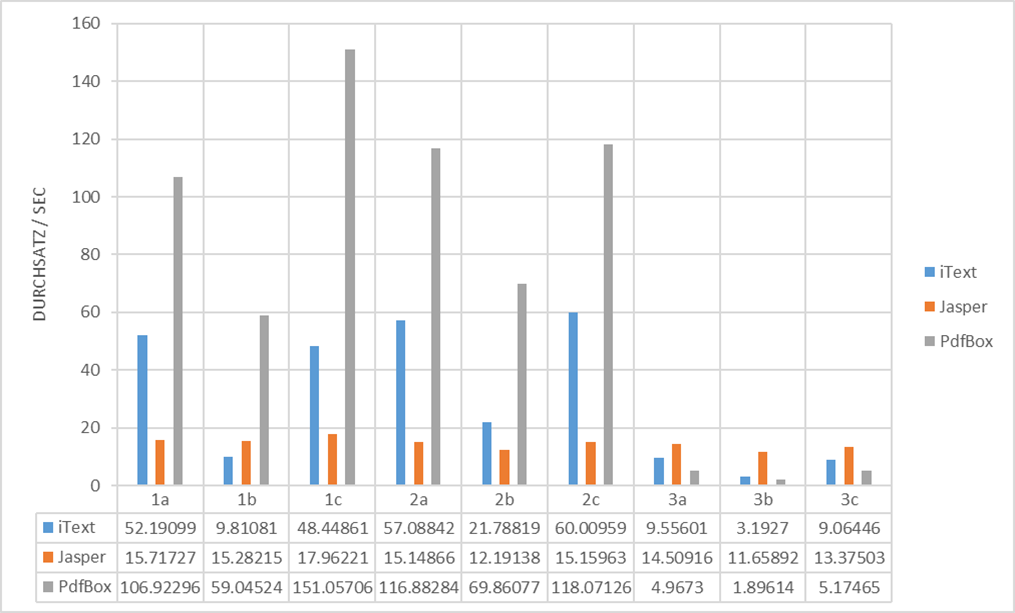
\includegraphics[width=\textwidth]{mainpart/4_analyse_img/VglDurchSzen.png}
 \caption{Vergleich - Durchsatz nach Szenario}
 \label{figure:throughputSzen}
\end{figure}

\subsection{Durchsatz nach Bytes}
Die Abbildung \ref{figure:throughputBytesAll} zeigt, dass der Durchsatz in Bytes über die Testdauer hinweg nicht Einbricht. Der Durchsatz nach Bytes scheint nur bei JasperReports tief zu bleiben. Der Durchsatz nach Bytes scheint auch bei Apache PDFBox und iText beim Szenario 3 zu steigen,  wobei der Durchsatz der Antworten nachlässt. Analyiert man die Grösse der Antworten wird auch klar warum. 
\begin{figure}[!h]
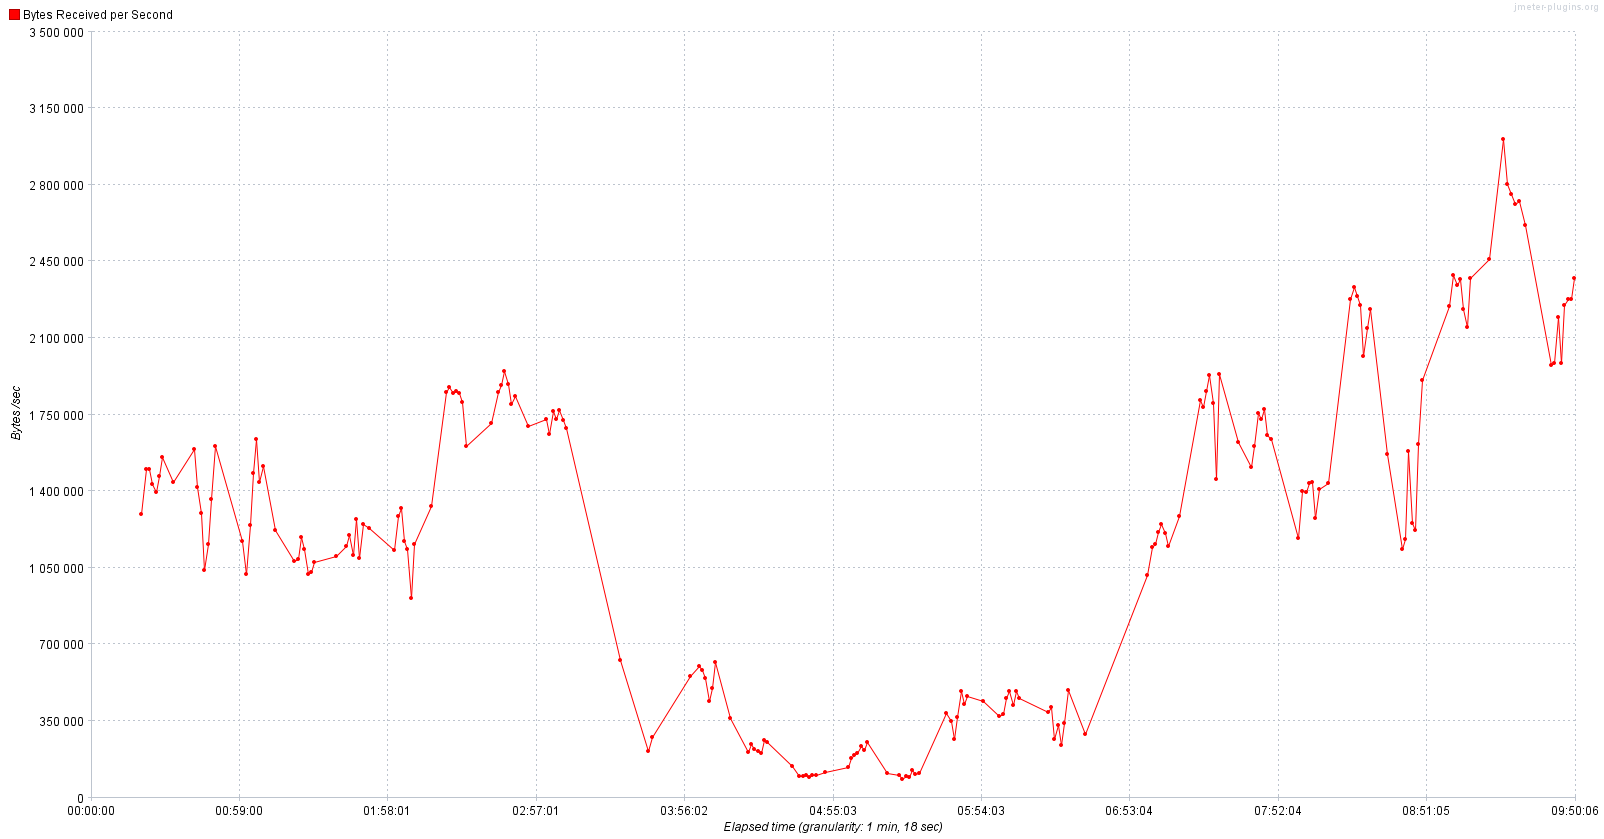
\includegraphics[width=\textwidth]{mainpart/4_analyse_img/ThroughputOverTimeAll.png}
 \caption{Durchsatz in Bytes}
 \label{figure:throughputBytesAll}
\end{figure}


% Diskussion verschoben werden
JasperReports generiert im Vergleich zu den anderen OSREs weitaus kleinere PDFs. Die Kontaktliste, eine Liste mit  Kontaktdaten und einem Gender-Symbol, die im Szenario 3 generiert wird, verarbeitet JasperReports besser als es die anderen OSREs. Es scheint als ob die Bilder referenziert und komprimiert werden, dies ist mithilfe der vorkompilierten Templates möglich. Das mit JasperReports generierten PDF ist etwa 46KB gross, das mit Apache PDFBox generierte PDF ist etwa 730KB gross. Etwas besser was die Komprimierung anbelangt kann bei iText beobachtet werden, mit iText wird das PDF etwa 350 KB gross.  
Dies bedeutet das zwar der Duchsatz nicht vergrössert wurde doch die generierten Files die Bandbreite des verfügbaren Netzwerkes dennoch genutzt wurde. Wie gross die Bandbreite eines Webservice ist und welche Netzwerkverbindung der Engpass darstellte konnte nicht festgestellt werden. 


\subsection{Latency}
%Min / Max Average --> Vergleichen mit anderen Projekten wer hat die kürzeste Latenz wer die längste
Die Latenzzeit die in der Abbildung \ref{figure:latencyTestcycle} dargestellt wird ist die Zeit die der Service gebraucht hat um die Anfrage zu bearbeiten samt Netzwerkzeit. 
% Diskussion
Diese Grafik korreliert klar mit der Analyse der Durchsätze. Der Durchsatz steigt umgekehrt proportional zur gemessen Latenzzeit. 


\begin{figure}[!ht]
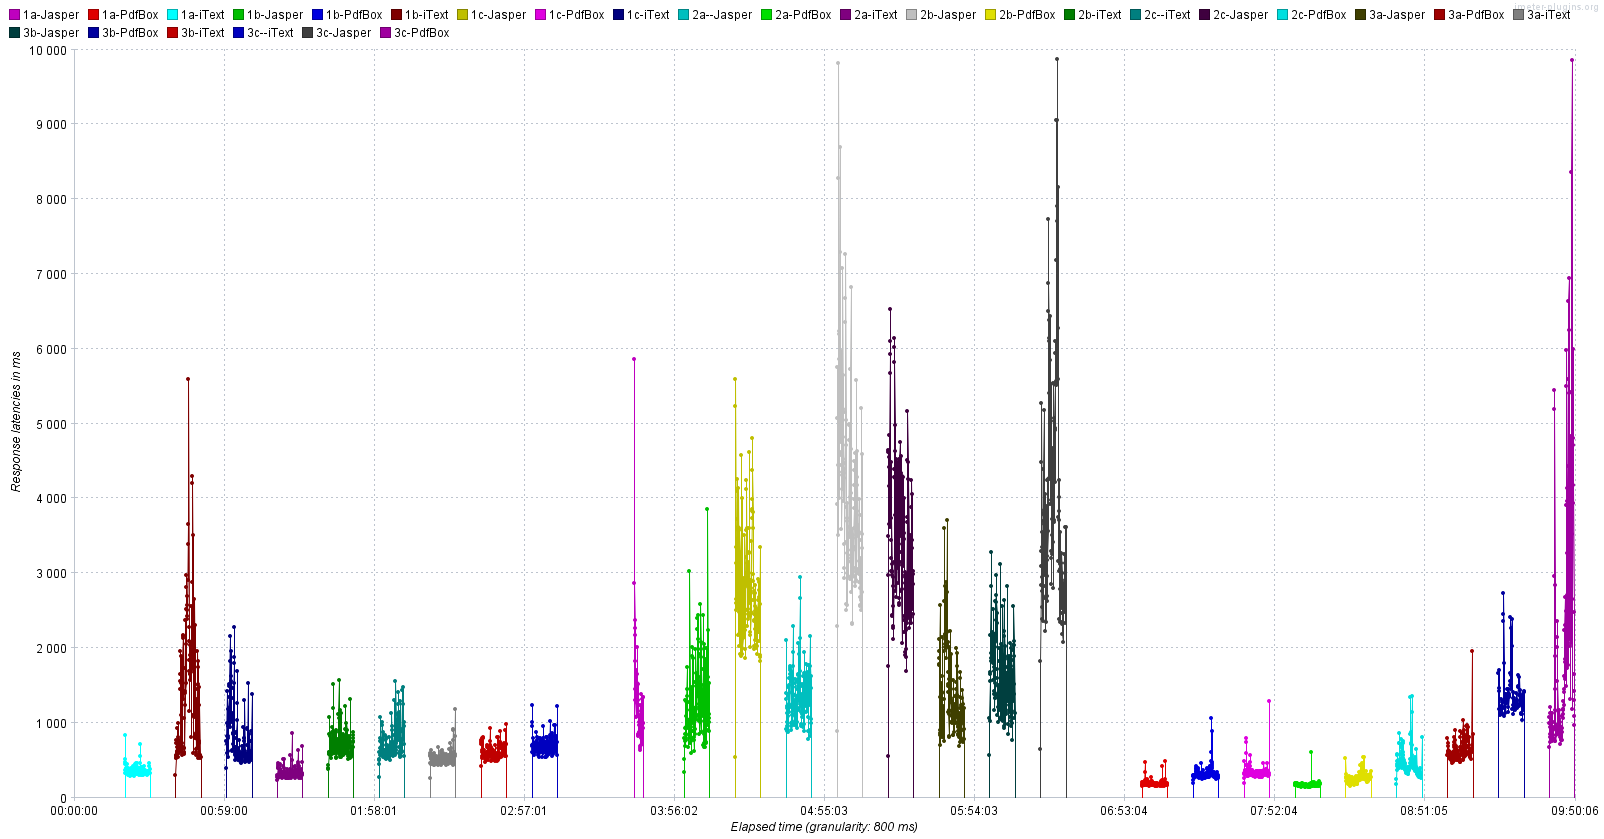
\includegraphics[width=\textwidth]{mainpart/4_analyse_img/ResponseLatenciesOverTime.png}
 \caption{Latenzzeit im Testzyklus}
 \label{figure:latencyTestcycle}
\end{figure}




Auch hier kommen iText und Apache PDFBox bei den meisten Szenarien mit weniger als einer Sekunde aus. Doch es sind auch Aussnahmen festzustellen, wie beim Szenario 1b bei iText und Szenario 3 bei Apache PDFBox. 
Diese Latenzzeiten sind keine Aussage zur Netzwerklatenz, die reine Zeit die verbraucht wird bis eine Nachricht vom Sender zum Empfänger übermittelt wurde. Diese Zeit gibt die Reine Antwortzeit des Service wieder. Wie auch die Abbdildung  \ref{figure:latencySzenario} vergrössert sich die Latenz wegen der Verarbeitungszeit währen dem Szenario 3. JasperReports zeigt dabei eine Überdurchschnittliche Latenzzeit wärend den ersten beiden Szenarien. 
% Diskussion
%% Der Serviec ist in den USA ist die Netzwerklatenz so gross um Hunderte oder sogar tausende von Antworten zu stoppen ? 

\begin{figure}[!ht]
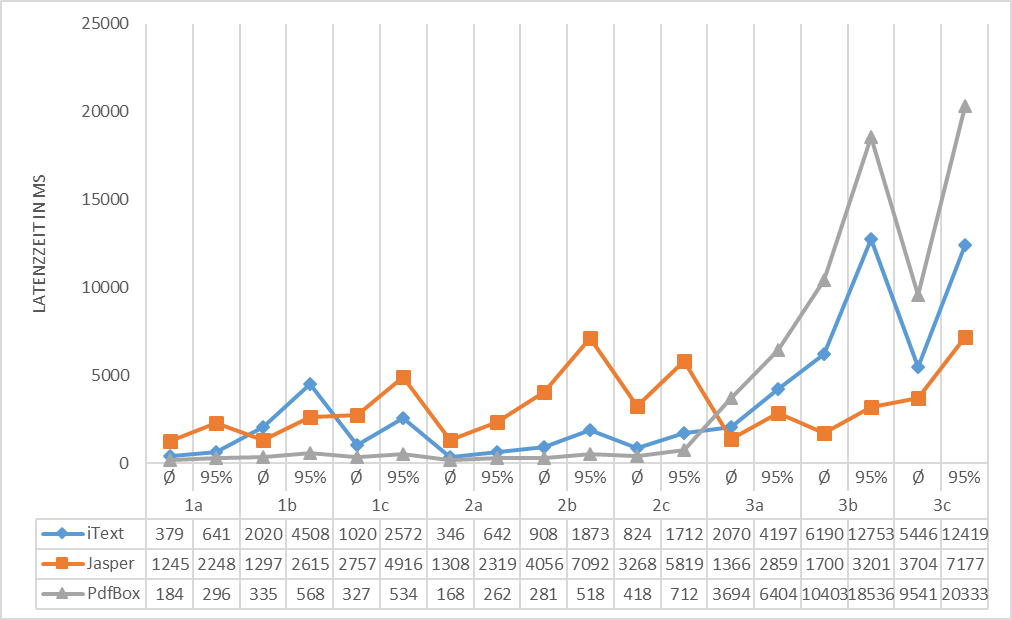
\includegraphics[width=\textwidth]{mainpart/4_analyse_img/LatenzzeitSzen.png}
 \caption{Latenzzeit nach Szenario und OSRE}
 \label{figure:latencySzenario}
\end{figure}

\subsection{Verfügbarkeit}

Der Service soll auch über die Zeit hinweg möglichst Verfügbar bleiben. Dies ist ebenfalls ein wichtiger Performance Indikator. Wären den Tests habt keiner der Services über den Testlauf von Rund drei Stunden einen Absturz gehabt oder ist unerreichbar gewesen. Die Prototypen waren im Verlauf der Test meist aktiv geblieben, was aber nicht heisst, dass ein User diese auch als Verfügbar empfunden hätte. Hätte man diese Prototypen im einer Produktionsumgebung eingesetzt wäre der User wohl des öfteren mit längeren Wartezeiten konfrontiert gewesen. Die Latenzzeiten die im vorgehenden  Kapitel erwähnt wurden wären auch hier ein Thema. In der Abbildung \ref{figure:latencySLA2000} wird ersichtlich wie viel Prozent der Anfragen an die entsprechenden Services länger gedauert hätte als 2 Sekunden. 

\begin{figure}[!ht]
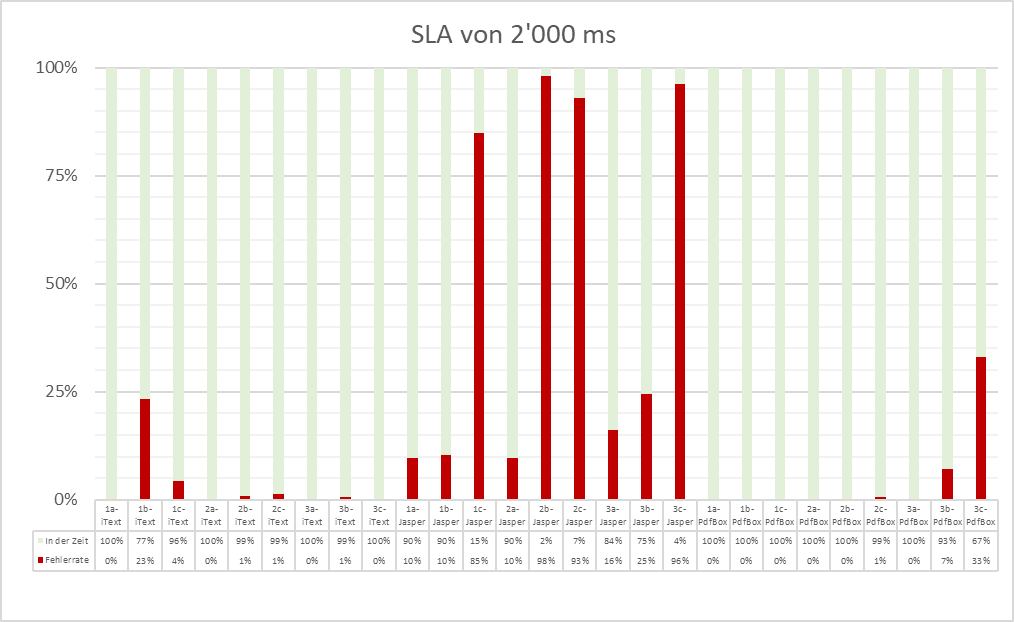
\includegraphics[width=\textwidth]{mainpart/4_analyse_img/latencySLA2000.png}
 \caption{Fehlerrate nach Latenzzeit über 2000ms}
 \label{figure:latencySLA2000}
\end{figure}


% Diskussion  oder Grundlagen?
Nach Molyneaux \cite[Kapitel~1]{molyneaux2014art} sind Verzögerungen erst dann ein Problem wenn diese mit dem Fluss der spezifischen Arbeit zusammenkommen. Ein Betriebssystem muss immer in weniger als 0.1 Sekunden antworten damit es den Arbeitsfluss nicht hindert. Auch hat ein Schreibprogramm in weniger als eine Sekunde zu reagieren auch wenn Graphiken verarbeitet werden, damit der User in seienm kreativen Prozess nicht gehindert wird. Weiter ist die Zeitspannen von 2 bis 4 Sekunden ebenfalls eine wichtige Grösse, bei komplexen Arbeiten bei denen der User sich Informationen merken muss ist es wichtig diese Antwortzeit so gering wie möglich zu halten. 

In der Abbildung \ref{figure:latencySLA2000} wird gezeigt dass für eine Online-Applikation besonder JasperRepots sich nicht wirklich eignete. Vier von neun Szenarien benötigen meisst mehr als 2 Sekunden um eine initiale Antwort zu senden. Die Latenzzeit ist ein mehr 85\% der ist Antworten benötigt mehr als 2 Sekunden. Dies wäre für den Online-Benutzer zu lange wären diese Daten für seinen Arbeitsprozess nötig.

JasperReports liefert 99\% der Antworten innerhalb von 10 Sekunden was für eine Batchverarbeitung akzeptabel wäre.
Dennoch hat auch iText und Apache PDFBox bei einer SLA von zwei Sekunden in einigen Fällen Schwierigkeiten. iText hat bei der Verarbeitung des Szenario 1b eine Verfügbarkeit von 77\% erreicht, was zu Tief ist für eine Online-Verarbeitung. Die übrigen Szenarien mit kleiner Aussnahme des Szenarios 1c der bei 96\%  angelangt ist konnte eine 99\% Antwortzeit von unter zwei Sekunden erreicht werden. 

Apache PDFBox zeigt hingegen wieder das die Verarbeitung der Reports im Szenario 3b und 3c oft eine Geschwindigkeit erreicht  die  für den User  nicht mehr angenehm oder akzeptabel empfinden würde. 









\section{Resourcen}

Welche Auswirkung die Test auf dem Webservern haben wird in den folgenden Kapitel behandelt. 

\subsection{Arbeitsspeicher}
Aus den Performancemessungen konnte der Verbrauch auf der PaaS geloggt werden und ist im der Abbildung \ref{figure:memorytestlauf} zu sehen. 
Die Memoryauslastung steigt bei der Ausführung der Performancetests und sinkt bei der Ausführung des GC oder einem Neustart des Webserver (Dyno). Die Dynos sind als Standard-X2 definiert, was bedeutet das die Maximale Auslastung auf den Memory RSS auf eine 1024MB beschränkt ist. Dies bedeutet dass die Auslastung auf dem Memory begrenzt ist und jede weitere verarbeitung auf den SWAP ausgelagert wird. 
Die Abbildung \ref{figure:memorytestlauf} zeigt dieses Phänomene. iText nutze nur wenig SWAP und konnte in den Performancetest meisst mit RSS Memory alle Anfragen bearbeiten. Ein Teil der Anfragen wurden dennoch im Szenario 3 im SWAP ausgelagert werden. 
Nach einem Restart des Webservices wurde JasperReports genutzt. Diese ORSE nutzte bereits das verfügbare Memory im ersten Szenario aus. Das Memory auf dem SWAP konnte über alle Szenarien hinweg nicht freigegeben werden was zu einem Aufblasen des Memoryverbrauch führte. JasperReport erreichte in Testlauf ein totaler Memoryverbrauch von 1389.32MB.
Apache PDFBox erreichte im Testlauf die Memory-Quota kaum. 


\begin{figure}[!ht]
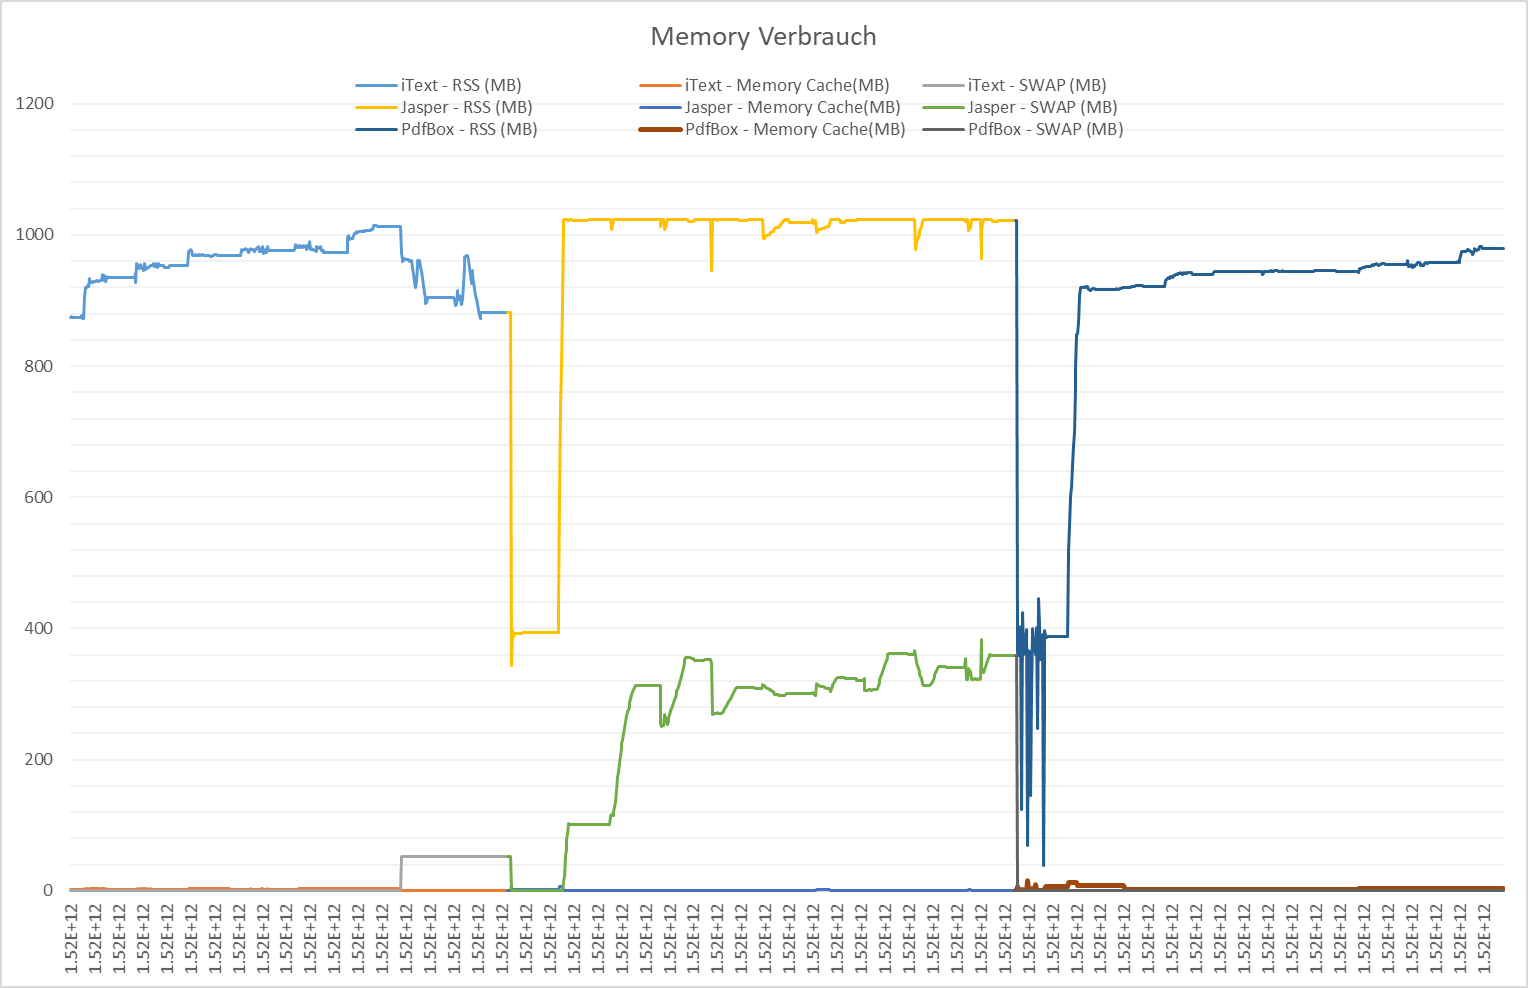
\includegraphics[width=\textwidth]{mainpart/4_analyse_img/MemoryVerbrauch.png}
 \caption{Memoryverbrauch Testlauf}
 \label{figure:memorytestlauf}
\end{figure}



\subsection{Prozessor Last}
Der Verbrauch des \acrlong{cpu}s ist eine etwas schwierige Messgrösse. Der \acrlong{paas} hat diese Daten mit der Stichprobengrösse einer Minute in die Logs geschrieben.

Dabei sind natürlich erkenntlich das im Textzyclus von iText die die Auslastung je nach Szenario sich sehr unterscheidet. Z.B. sind während dem zweiten Szenario Durchschnittlich  zwischen vier und sieben Prozessor im Status 'Ready' pendent gewesen. Hingegen sind im dritten Szenario fast immer alles Prozessoren in Ausführung gewesen das bedeutet eine fast optimale Auslastung des CPUs mit wenige wartende Prozessen. Wiederum sind diese wohl so entstanden da die Prozesse im dritten Szenario langläufiger gewesen sind und somit wenig neue Anfragen verarbeitet worden. 

JaspeRepors hat den CPU eher gefordert und hat durch den ganzen Zeitraum viele Prozesse gebraucht. Wie intensiv die Verarbeitung von JasperReports im Vergleich zu den anderen OSREs wird hier klar hervorgehoben. 

Apache PDFBox ist hier als sparsamster \acrlong{osre} zu erkennen. Es wurden maximal fünf Prozesse ausgelagert. 
\begin{figure}[!hb]
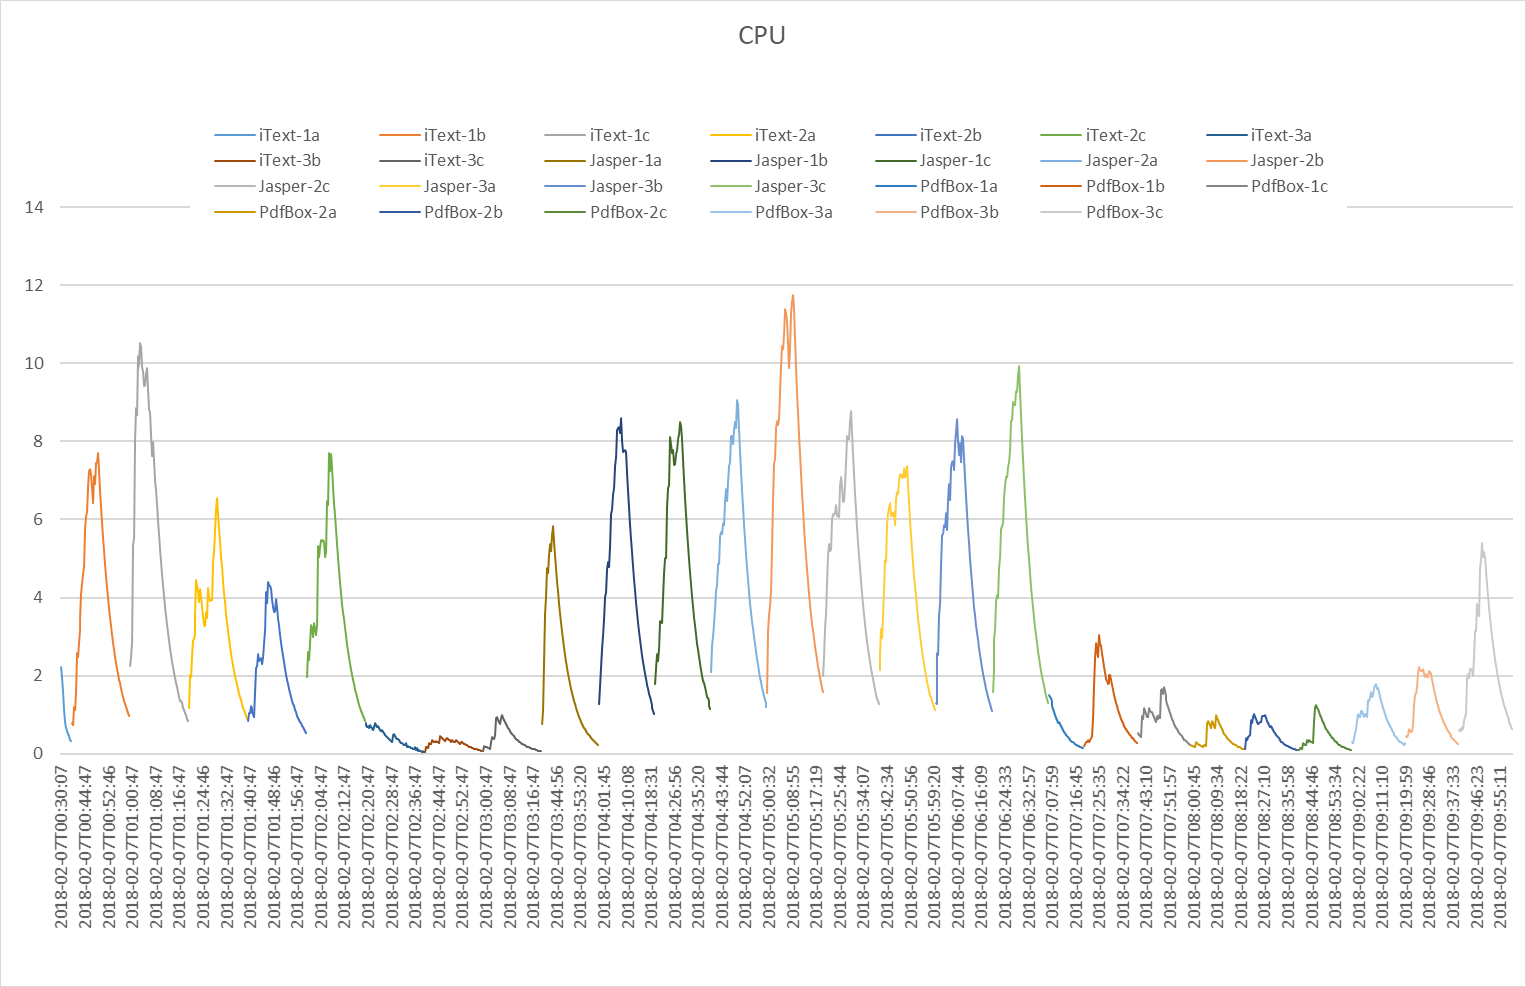
\includegraphics[width=\textwidth]{mainpart/4_analyse_img/CPUVergleich.png}
 \caption{Vergleich - Durchsatz nach Szenario}
 \label{figure:cpuVergleich}
\end{figure}




\section{Reporting Engines - Verhalten}


Die OSRE haben sich während den Test, in Bezug auf die Lastveränderung verschieden verhalten. In diesem Kapitel sollen die Veränderungen von Requestgrössen und der Zunahme von \acrfull{vu} weiter aufgezeigt werden. 

\subsection{Requestgrösse}

Im Vergleich zu den Szenarien 1a, 2a und 3a wurden bei den Szenarien 1b, 2b und 3b die Datensätze für die Verarbeitung verdreifacht. Wie aus der Abbildungen \ref{figure:vglABRequ} entnommen werden kann hat die dazu geführt das sich alle Antwortzeiten und Durchsätze verschlechtert haben.

\begin{figure}[!hb]
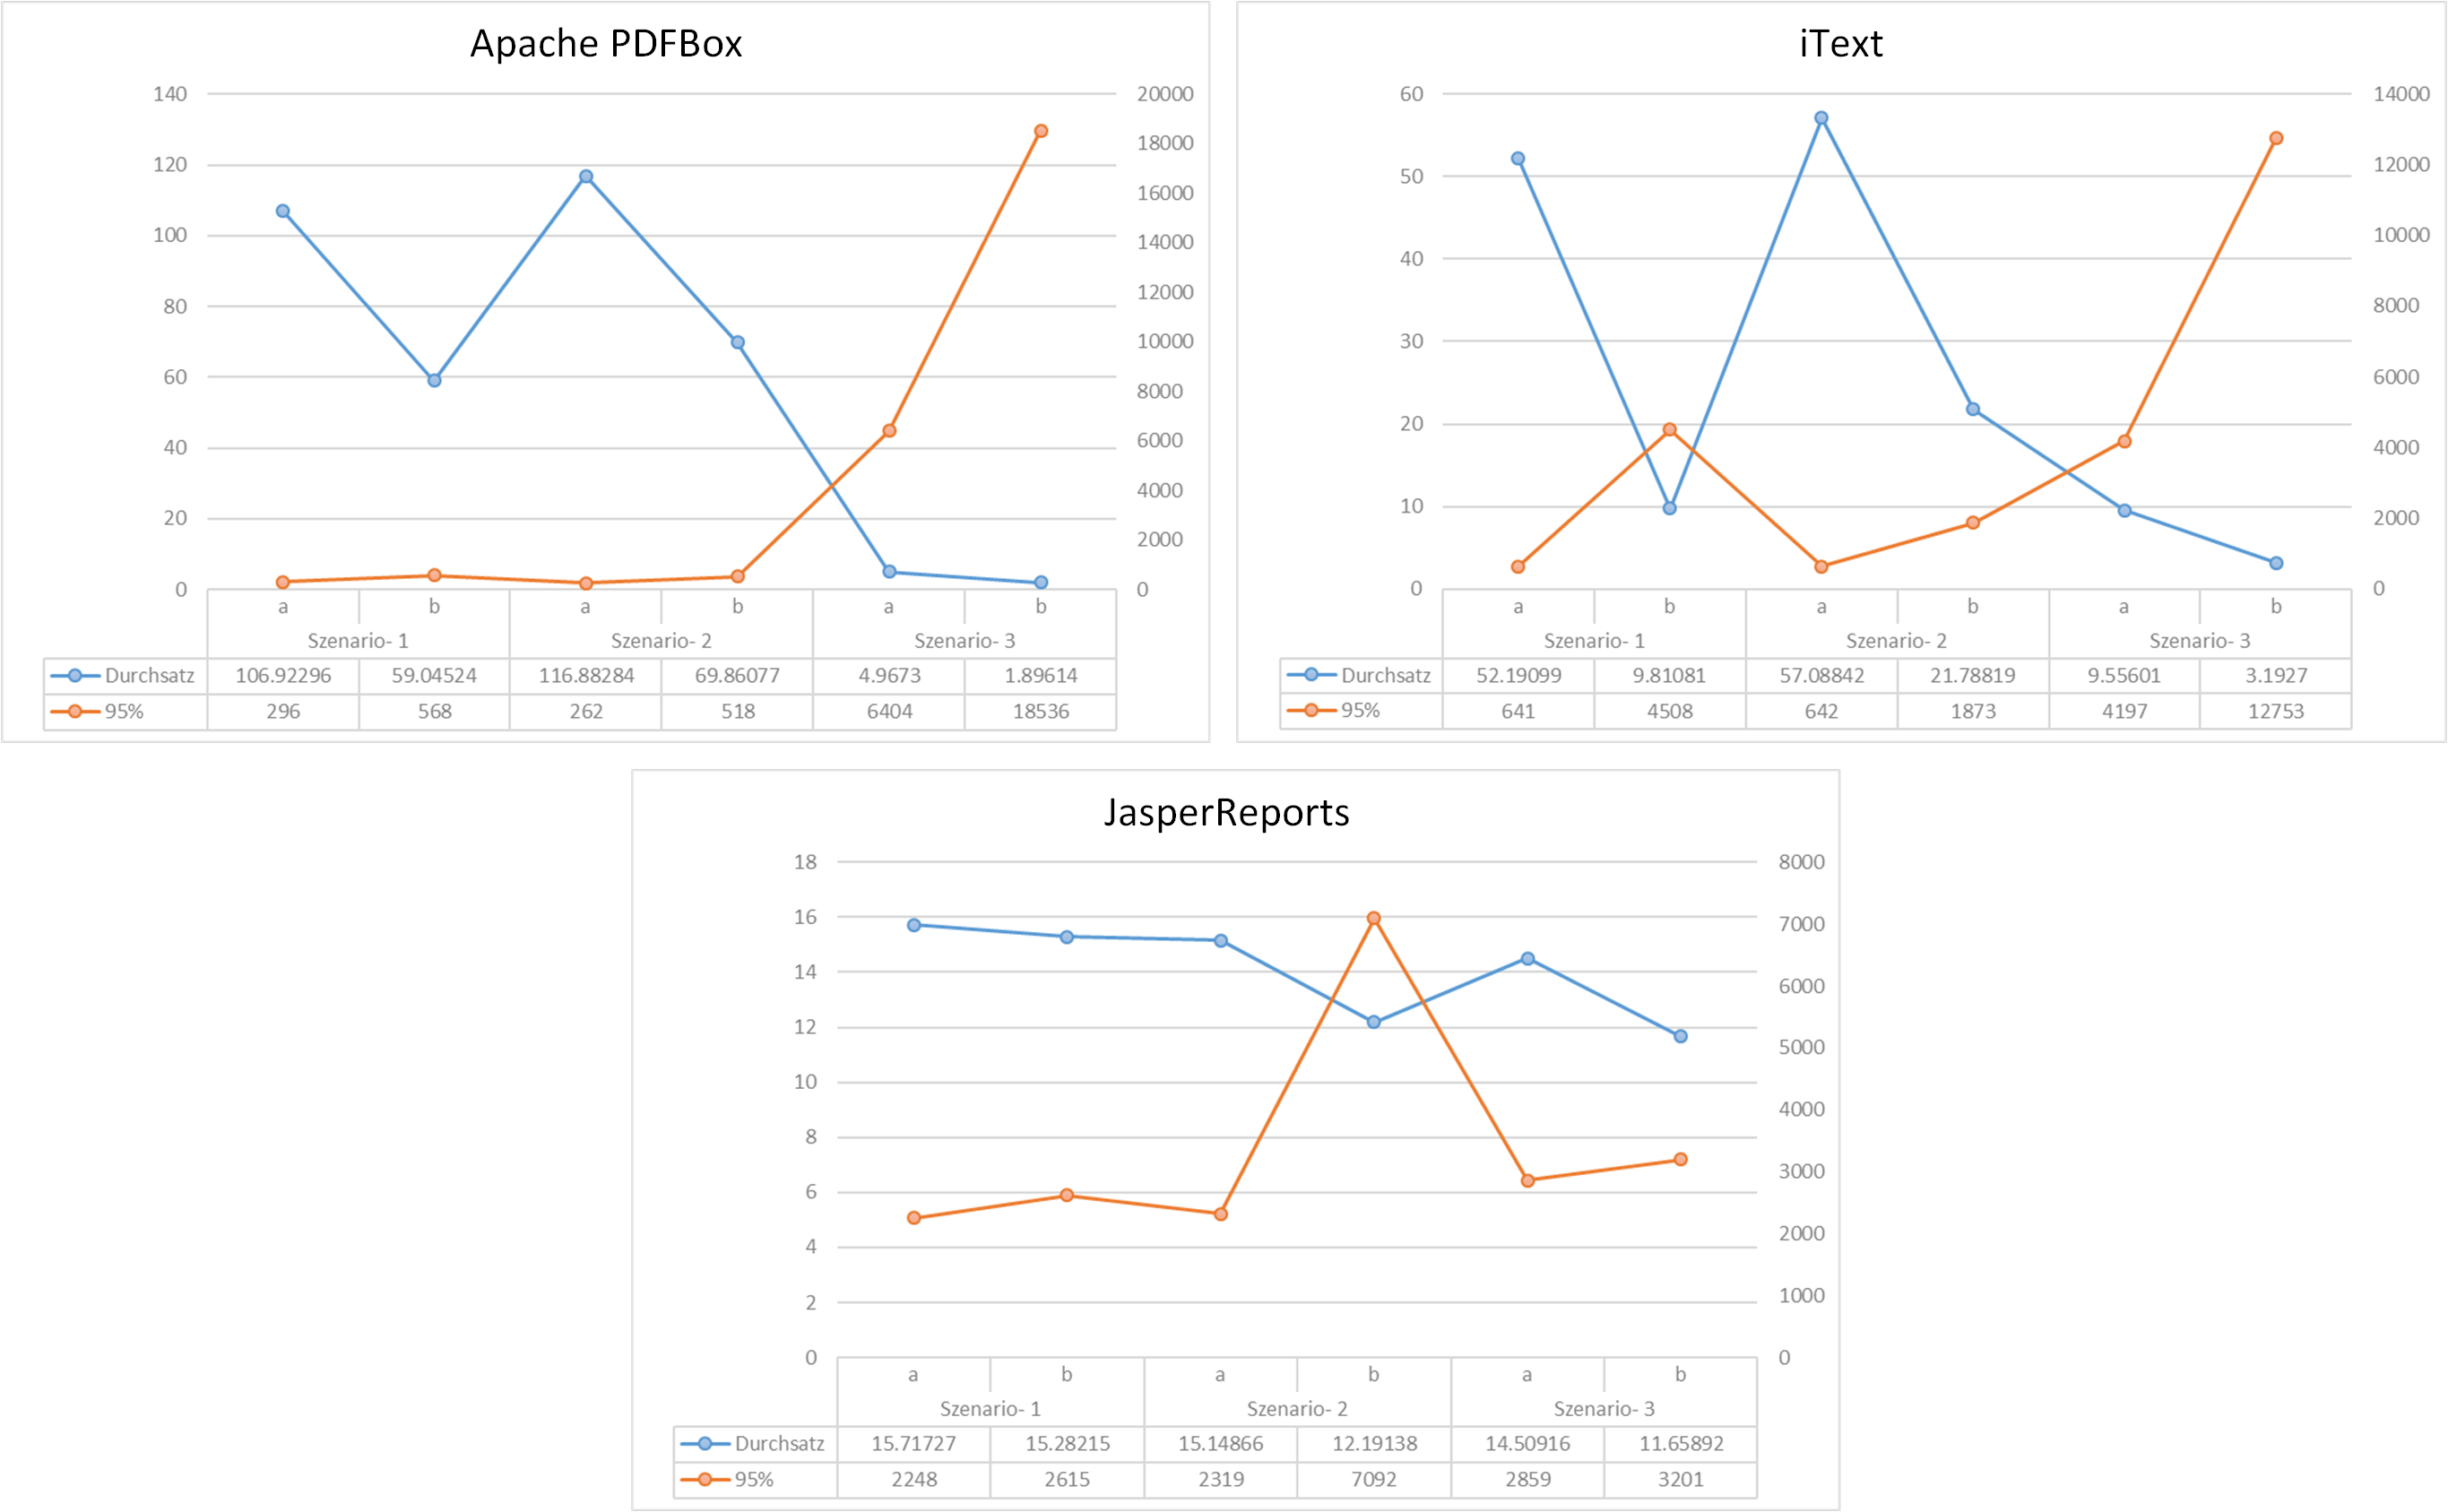
\includegraphics[width=\textwidth]{mainpart/4_analyse_img/ABAuswertung.png}
 \caption{Vergleich Baseline mit grösserer Datenmengen}
 \label{figure:vglABRequ}
\end{figure}

Die OSRE und iText und Apache PDFBox haben sich in der gleichen Art und Weise verschlechtert. iText verzeichnet hier  Durchsatzeinbrüche. Die ersten zwei Szenarien fallen je von zwischen 50 und 60 auf  fast 10 und 21 Anfragen pro Sekunde. 

Hier sei noch einmal hervorgehoben dass diese Daten aufgrund eines Testlaufs ermittelt wurden, es kann in jedem Testlauf das gleiche Phänomen beobachtet werden, dennoch sind diese Daten nicht stellvertretend oder absolut zu betrachten, grösserer Ausreisser wurden in anderen Testläufe aufgezeichnet.





\subsection{Virtuelle User}
Die Prototypen wurden  von den initialen 20 \acrfull{vu} im Szenario 'a' weiter gefordert als 30 weitere \acrshort{vu}s hinzugefügt wurden um eine erhöhte Nutzerinteraktionen zu simulieren. Wie die \acrlong{osre}s dabei reagiert haben kann aus der Abbildung \ref{figure:vglACVU} gesehen werden. In den Abbildungen werden die Veränderung des Durchsatzes mit dem 95 Perzentil der Antwortzeit verglichen. Dabei ist nur massgebend wie sich die OSRE im Durchschnitt verhalten. 

\begin{figure}[!ht]
\includegraphics[width=\textwidth]{mainpart/4_analyse_img/ACAuswertung.png}
 \caption{Vergleich Baseline mit mehr virtuellen Usern}
 \label{figure:vglACVU}
\end{figure}

Einige der interessanten Erkenntnisse in diesem Zusammenhang kann kann bei Apache PDFBox entdeckt werden. Obwohl die Nutzerlast steigt, steigt auch der Durchsatz im Szenario 1 von 106 auf 151 Anfragen pro Sekunde. Die Antwortzeit verdoppelt sich aber dabei. Ähnliches ist auch im zweiten Szenario zu beobachten. Einen Kreuzvergleich mit der Zuname der zu verarbeitenden Daten (Abbildung \ref{figure:vglABRequ}) sieht man klar das diese im Durchsatz einen klaren Einbruch erleben aber die Antwortzeit gleich blieb. Apache PDFBox hat klar mühe mit dem Szenario 3 die Antwortzeit verdreifacht sich dabei wobei der Durchsatz gleich bleibt.

iText scheint in der Implementation der ersten zwei Szenarien ähnliches Verhalten unter Last zu erzeugen. Die Antwortzeit wird im ersten Szenario vier mal langsamer Szenario 2 eine drei mal langsamere Antwortzeit. Auch iText schafft es seine Durchsatz zu verbessern und zwar im Szenario werden drei Antworten mehr pro Sekunde verarbeitet. Szenario 3 hat ähnliche Probleme wie Apache PDFBox die Antwortzeiten verdreifachen sich und der Durchsatz bleibt auch bei iText etwa konstant.

JasperReports verschlechtert sich in allen Antwortzeiten aber nicht ganz so extrem wie iText und Apache PDFBox, in allen Szenarien verschlechtern sich die Antwortzeiten. Etwa bei allen Szenarien wurde JasperReports etwa doppelt so langsam. Was der Durchsatz anbelangt blieb dieser fast konstant, im Szenario 1 wurde dieser ebenfalls etwas höher (2 Anfragen pro Sekunde mehr) . 




\section{Ursachenanalyse}

Im Szenario 3 konnte man den Rückgang von iText und Apache PDFBox erkennen. Es lässt sich anhand der Ergebnisse der verschiedenen Metriken die  Schlussfolgerung gezogen werden, dass der Durchsatz nicht durch eine Netzwerk- oder Infrastrukturstörung herbeigeführt wurde. Es ist fraglich ob das sich diese schlechte Performance einen Zusammehang mit anderen nicht beinflussbaren Einflussfaktoren haben können. Dennoch zeigt sich einerseits das die Implementierung im Zusammenhang mit dem Szenario 3 zur Generierung von Vergleichsweise grossen PDFs führte. andererseits ist der Aufbau und Layout bei iText und Apache PDFBox mit mehr Rechenleistung verbunden. Apache PDFBox zeigt bei der Last auf dem PaaS-Provider höhere Last bei der Ausführung des Szenario 3. iText wiederum zeigt keine Zuname sondern sogar einen Rückgang der CPU-Last. 

Bei der Analyse mittels Java visual VM wurde entnommen das bei der Ausführung von JasperReports viele Objekte angelegt werden die im Zusammenhang mit den Jasper-Template stehen. Jedes Feld wird dabei ausgelesen und als Ressource gehalten. 

\end{document}